\documentclass[12pt,letterpaper]{article}
\usepackage{graphicx,textcomp}
\usepackage{natbib}
\usepackage{setspace}
\usepackage{fullpage}
\usepackage{color}
\usepackage[reqno]{amsmath}
\usepackage{amsthm}
\usepackage{fancyvrb}
\usepackage{amssymb,enumerate}
\usepackage[all]{xy}
\usepackage{endnotes}
\usepackage{lscape}
\newtheorem{com}{Comment}
\usepackage{float}
\usepackage{hyperref}
\newtheorem{lem} {Lemma}
\newtheorem{prop}{Proposition}
\newtheorem{thm}{Theorem}
\newtheorem{defn}{Definition}
\newtheorem{cor}{Corollary}
\newtheorem{obs}{Observation}
\usepackage[compact]{titlesec}
\usepackage{dcolumn}
\usepackage{tikz}
\usetikzlibrary{arrows}
\usepackage{multirow}
\usepackage{xcolor}
\newcolumntype{.}{D{.}{.}{-1}}
\newcolumntype{d}[1]{D{.}{.}{#1}}
\definecolor{light-gray}{gray}{0.65}
\usepackage{url}
\usepackage{listings}
\usepackage{color}

\definecolor{codegreen}{rgb}{0,0.6,0}
\definecolor{codegray}{rgb}{0.5,0.5,0.5}
\definecolor{codepurple}{rgb}{0.58,0,0.82}
\definecolor{backcolour}{rgb}{0.95,0.95,0.92}

\lstdefinestyle{mystyle}{
	backgroundcolor=\color{backcolour},   
	commentstyle=\color{codegreen},
	keywordstyle=\color{magenta},
	numberstyle=\tiny\color{codegray},
	stringstyle=\color{codepurple},
	basicstyle=\footnotesize,
	breakatwhitespace=false,         
	breaklines=true,                 
	captionpos=b,                    
	keepspaces=true,                 
	numbers=left,                    
	numbersep=5pt,                  
	showspaces=false,                
	showstringspaces=false,
	showtabs=false,                  
	tabsize=2
}
\lstset{style=mystyle}
\newcommand{\Sref}[1]{Section~\ref{#1}}
\newtheorem{hyp}{Hypothesis}

\title{Problem Set 3}
\date{Due: November 11, 2024}
\author{Applied Stats/Quant Methods 1
	\\ Jia Lyu-2337006}


\begin{document}
	\maketitle
	\section*{Instructions}
	\begin{itemize}
		\item Please show your work! You may lose points by simply writing in the answer. If the problem requires you to execute commands in \texttt{R}, please include the code you used to get your answers. Please also include the \texttt{.R} file that contains your code. If you are not sure if work needs to be shown for a particular problem, please ask.
	\item Your homework should be submitted electronically on GitHub.
	\item This problem set is due before 23:59 on Sunday November 11, 2024. No late assignments will be accepted.

	\end{itemize}

		\vspace{.25cm}
	
\noindent In this problem set, you will run several regressions and create an add variable plot (see the lecture slides) in \texttt{R} using the \texttt{incumbents\_subset.csv} dataset. Include all of your code.

	\vspace{.5cm}
\section*{Question 1}
\vspace{.25cm}
\noindent We are interested in knowing how the difference in campaign spending between incumbent and challenger affects the incumbent's vote share. 
	\begin{enumerate}
		\item Run a regression where the outcome variable is \texttt{voteshare} and the explanatory variable is \texttt{difflog}.
			\lstinputlisting[language=R, firstline=38, lastline=40]{PS3_Lyu_Jia.R}  
			\begin{verbatim} 
			Call:
			lm(formula = voteshare ~ difflog, data = df)
			
			Residuals:
			  Min       1Q      Median     3Q      Max 
			-0.26832 -0.05345 -0.00377  0.04780  0.32749 
			
			Coefficients:
			            Estimate Std. Error t value Pr(>|t|)    
			(Intercept) 0.579031   0.002251  257.19   <2e-16 ***
			difflog        0.041666   0.000968   43.04   <2e-16 ***
			---
			Signif. codes:  0 ‘***’ 0.001 ‘**’ 0.01 ‘*’ 0.05 ‘.’ 0.1 ‘ ’ 1
			
			Residual standard error: 0.07867 on 3191 degrees of freedom
			Multiple R-squared:  0.3673,	Adjusted R-squared:  0.3671 
			F-statistic:  1853 on 1 and 3191 DF,  p-value: < 2.2e-16
	 	
			The regression analysis reveals that the difference in 
			campaign  spending (`difflog`) explains a moderate 
			portion (36.73%) of the variability in the incumbent's vote 
			share   (`voteshare`). With a R-squared of 0.3673 and an 
			adjusted  R-squared of 0.3671, the model suggests that 
			`difflog` contributes meaningfully to predicting vote share 
			without indicating overfitting. The residual standard error 
			(0.07867) indicates a relatively close fit between observed 
			and predicted values. 
			A highly significant F-statistic (1853, p < 2.2e-16) further 
			confirms the model’s relevance, underscoring `difflog` as 
			a statistically significant predictor of `voteshare`, although
			other factors may also play a role.
		\end{verbatim}	
		
		
		\item Make a scatterplot of the two variables and add the regression line. 	
		\lstinputlisting[language=R, firstline=42, lastline=48]{PS3_Lyu_Jia.R}  
		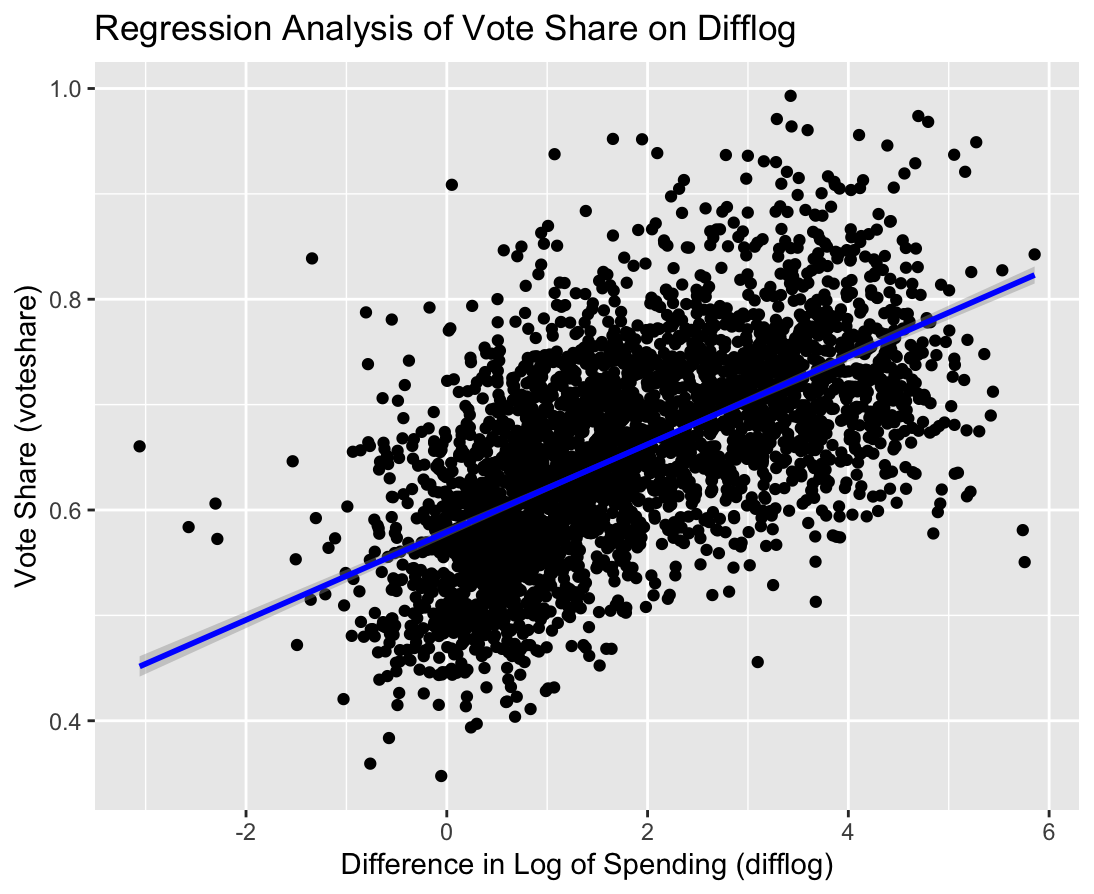
\includegraphics[width=.80\textwidth]{Scatterplot_1.2.png}
		
		\item Save the residuals of the model in a separate object.	
		\lstinputlisting[language=R, firstline=51, lastline=54]{PS3_Lyu_Jia.R}  
	
			\begin{verbatim}
		 1             2             3            
		-0.0004227622 -0.0316840149 -0.0045514943  
		 4             5             6 
		0.0386688767  0.0355287965   0.0322832521 
		
			\end{verbatim}	
		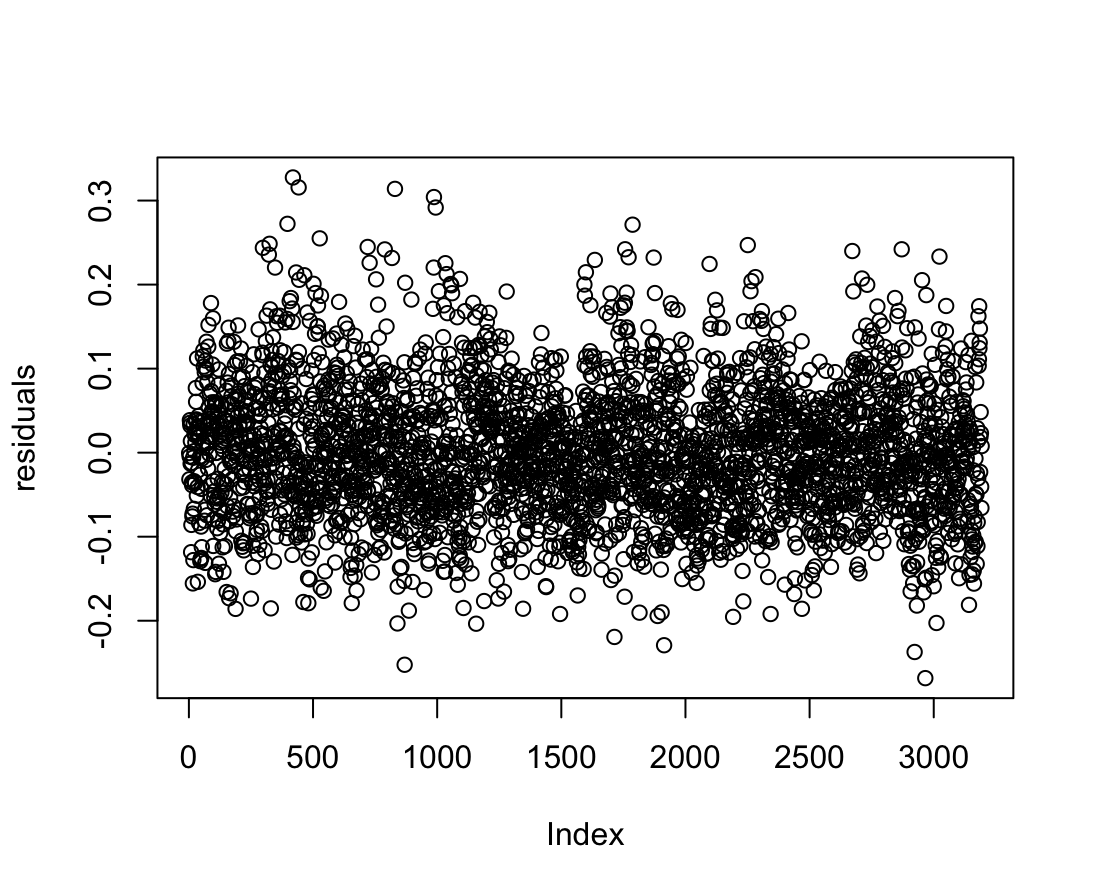
\includegraphics[width=.80\textwidth]{Scatterplot_1.3.png}
		\item Write the prediction equation.
		\lstinputlisting[language=R, firstline=57, lastline=63]{PS3_Lyu_Jia.R}  
		\begin{verbatim}
		"voteshare = 0.579030710920674  +  0.0416663238227399 * difflog"
	\end{verbatim}	
	\end{enumerate}
	
\newpage

\section*{Question 2}
\noindent We are interested in knowing how the difference between incumbent and challenger's spending and the vote share of the presidential candidate of the incumbent's party are related.	\vspace{.25cm}
	\begin{enumerate}
		\item Run a regression where the outcome variable is \texttt{presvote} and the explanatory variable is \texttt{difflog}.	
		\lstinputlisting[language=R, firstline=66, lastline=67]{PS3_Lyu_Jia.R}  
		\begin{verbatim}
		Call:
		lm(formula = presvote ~ difflog, data = df)
		
		Residuals:
		Min       1Q   Median       3Q      Max 
		-0.32196 -0.07407 -0.00102  0.07151  0.42743 
		
		Coefficients:
		Estimate Std. Error t value Pr(>|t|)    
		(Intercept) 0.507583   0.003161  160.60   <2e-16 ***
		difflog     0.023837   0.001359   17.54   <2e-16 ***
		---
		Signif. codes:  0 ‘***’ 0.001 ‘**’ 0.01 ‘*’ 0.05 ‘.’ 0.1 ‘ ’ 1
		
		Residual standard error: 0.1104 on 3191 degrees of freedom
		Multiple R-squared:  0.08795,	Adjusted R-squared:  0.08767 
		F-statistic: 307.7 on 1 and 3191 DF,  p-value: < 2.2e-16
		\end{verbatim}	\begin{verbatim}
		The regression analysis reveals a significant positive relationship 
		between the difference in campaign spending (`difflog`) and the incumbent’s 
		vote share (`presvote`). Specifically, for every one-unit increase in    
		`difflog`, the incumbent’s vote share increases  by approximately 
		0.023837 units. The model’s intercept is 0.507583, with both the
		intercept and the slope being statistically significant 
		(p-value < 2e-16). The coefficient of determination (R-squared) is
		0.08795, indicating that about 8.8% of the variation in the incumbent’s
		vote share can be explained by the difference in campaign spending.
		Although the model is statistically significant (F-statistic = 307.7, 
		p-value < 2.2e-16), its explanatory power is limited, suggesting that 
		other factors beyond campaign spending may also influence the incumbent’s 
		vote share.
		\end{verbatim}	
		
		\item Make a scatterplot of the two variables and add the regression line. 	\lstinputlisting[language=R, firstline=69, lastline=75]{PS3_Lyu_Jia.R}  
			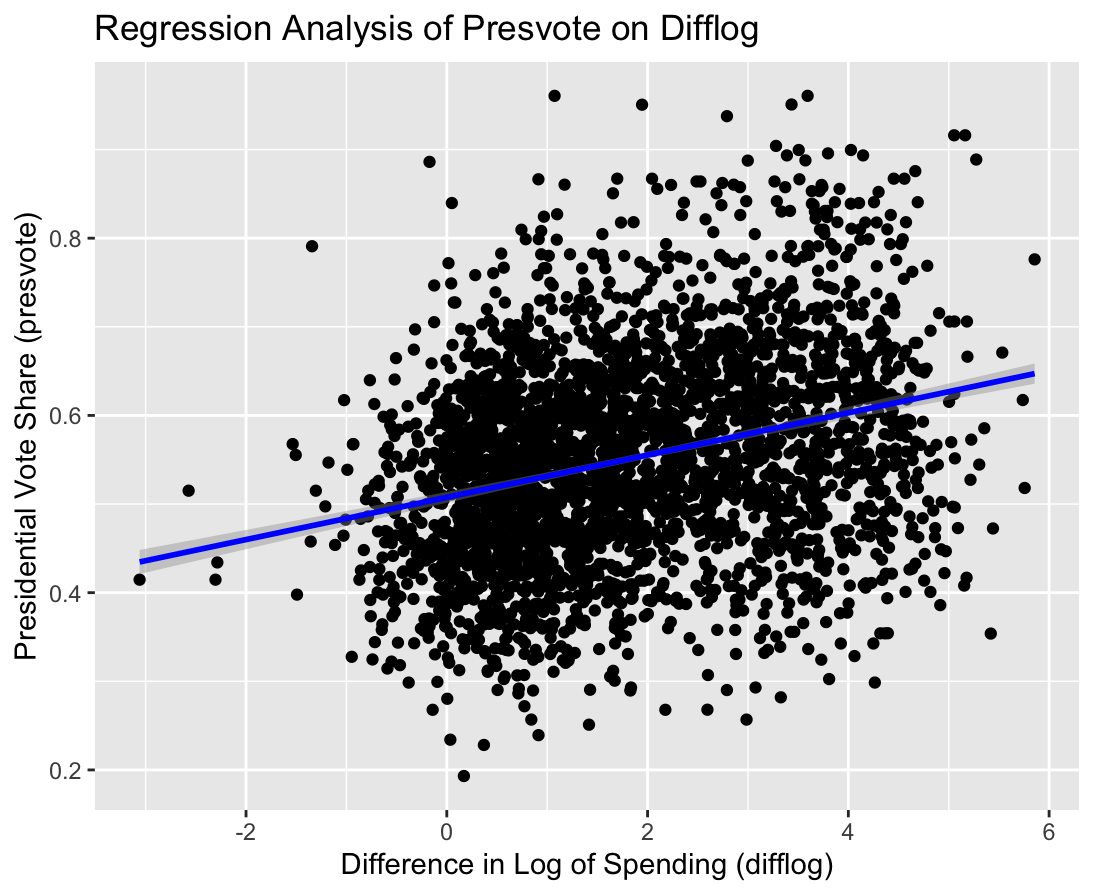
\includegraphics[width=.80\textwidth]{Scatterplot_2.2.png}
		\item Save the residuals of the model in a separate object.	
		\lstinputlisting[language=R, firstline=77, lastline=84]{PS3_Lyu_Jia.R}  
		\vspace{.2cm}
		\begin{verbatim}
		 1            2            3            4            5            6 
		0.005605594  0.037578519 -0.053134788 -0.052993694 -0.045842994  0.074339701
		\end{verbatim}	
		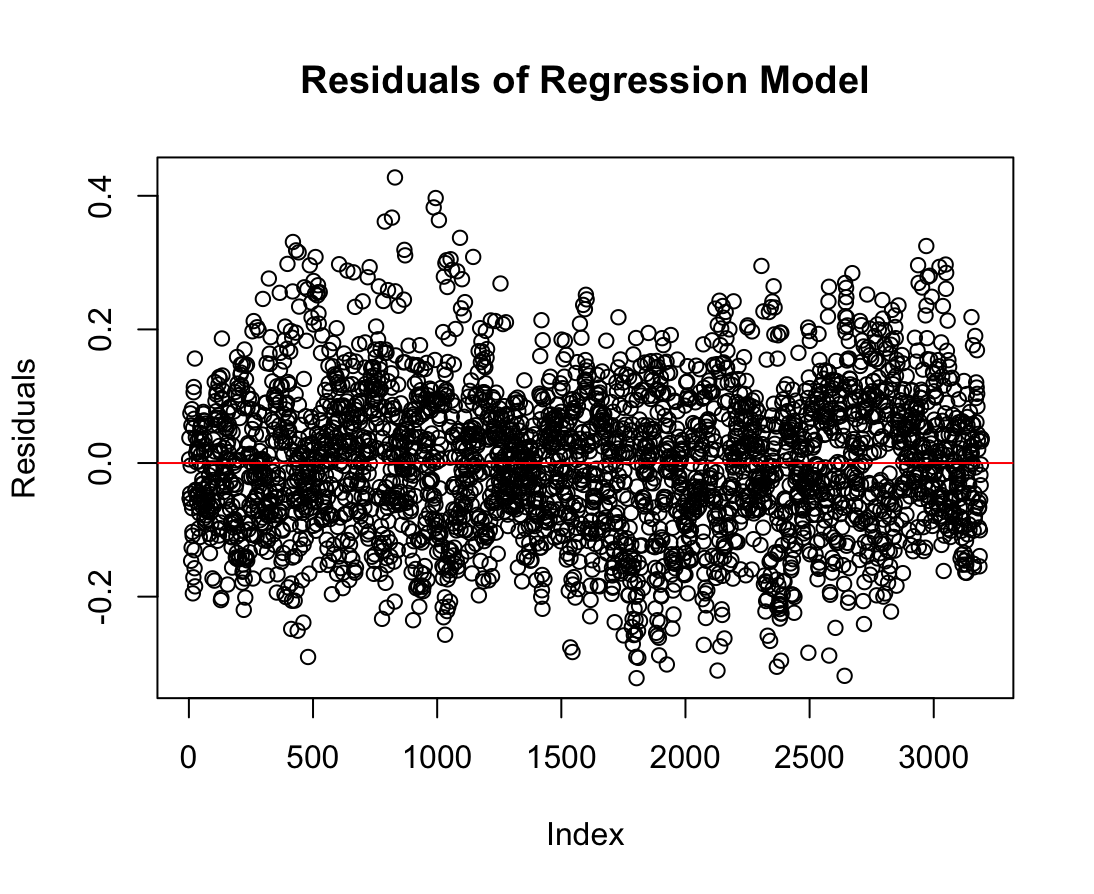
\includegraphics[width=.80\textwidth]{Scatterplot_2.3.png}
		 
		\item Write the prediction equation.
		\lstinputlisting[language=R, firstline=86, lastline=91]{PS3_Lyu_Jia.R} 
		\begin{verbatim}
		"presvote = 0.508  +  0.024 * difflog"
		 	\end{verbatim}	
	\end{enumerate}
	
	\newpage	
\section*{Question 3}

\noindent We are interested in knowing how the vote share of the presidential candidate of the incumbent's party is associated with the incumbent's electoral success.
	\vspace{.25cm}
	\begin{enumerate}
		\item Run a regression where the outcome variable is \texttt{voteshare} and the explanatory variable is \texttt{presvote}.
			\lstinputlisting[language=R, firstline=94, lastline=96]{PS3_Lyu_Jia.R} 
				\begin{verbatim}
			Call:
			lm(formula = voteshare ~ presvote, data = df)
			
			Residuals:
			Min       1Q   Median       3Q      Max 
			-0.27330 -0.05888  0.00394  0.06148  0.41365 
			
			Coefficients:
			Estimate Std. Error t value Pr(>|t|)    
			(Intercept) 0.441330   0.007599   58.08   <2e-16 ***
			presvote    0.388018   0.013493   28.76   <2e-16 ***
			---
			Signif. codes:  0 ‘***’ 0.001 ‘**’ 0.01 ‘*’ 0.05 ‘.’ 0.1 ‘ ’ 1
			
			Residual standard error: 0.08815 on 3191 degrees of freedom
			Multiple R-squared:  0.2058,	Adjusted R-squared:  0.2056 
			F-statistic:   827 on 1 and 3191 DF,  p-value: < 2.2e-16
				\end{verbatim}	
				\begin{verbatim}
			The regression analysis reveals a significant positive relationship 
			between `presvote` and the incumbent’s `voteshare`. Specifically, 
			for every one-unit increase in the presidential vote share, the incumbent’s 
			vote share increases by approximately 0.2465. 
			The model explains about 8.7% of the variability in the incumbent's 
			vote share, suggesting that other factors beyond `presvote` may 
			also influence the incumbent's electoral success.
						\end{verbatim}	
		\item Make a scatterplot of the two variables and add the regression line. 
			\lstinputlisting[language=R, firstline=98, lastline=105]{PS3_Lyu_Jia.R} 
				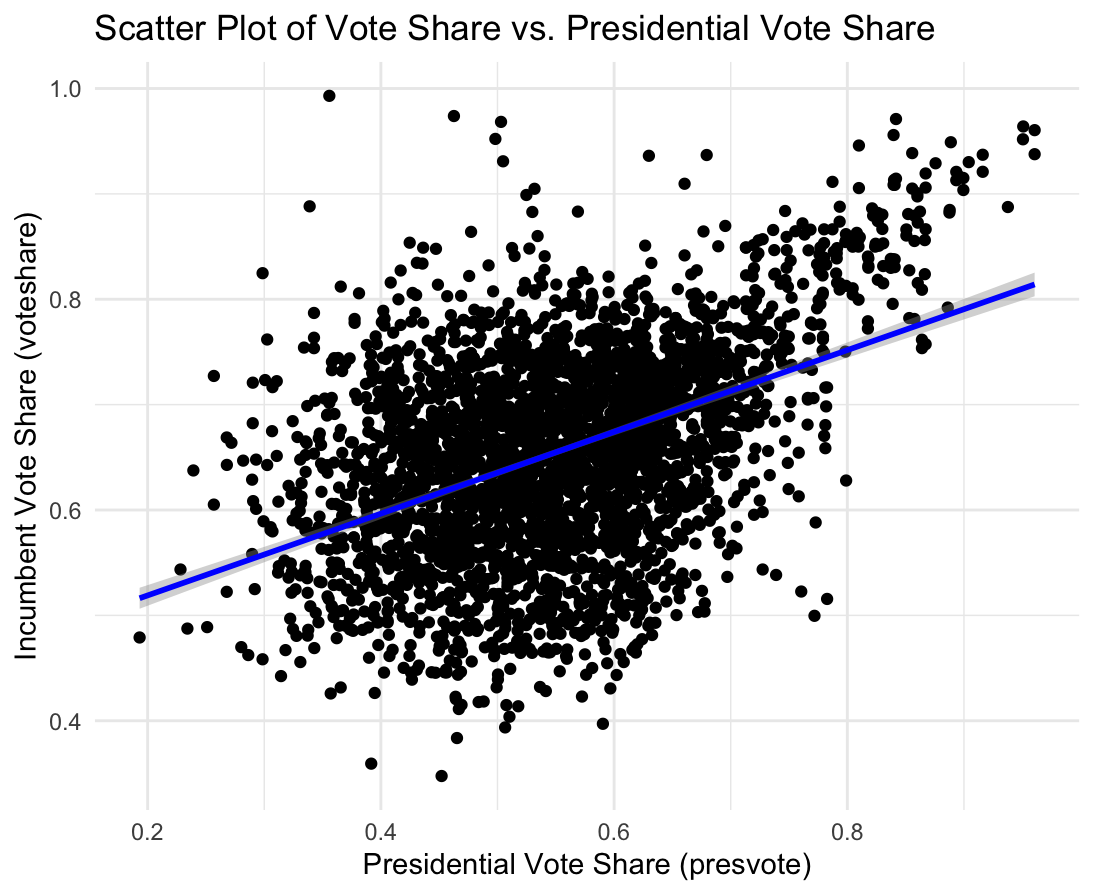
\includegraphics[width=.80\textwidth]{Scatterplot_3.2.png}
		\item Write the prediction equation.
		\lstinputlisting[language=R, firstline=106, lastline=111]{PS3_Lyu_Jia.R} 
		\begin{verbatim}
			"voteshare = 0.441  +  0.388 * presvote"
	\end{verbatim}	
		\end{enumerate}

\newpage	
\section*{Question 4}
\noindent The residuals from part (a) tell us how much of the variation in \texttt{voteshare} is $not$ explained by the difference in spending between incumbent and challenger. The residuals in part (b) tell us how much of the variation in \texttt{presvote} is $not$ explained by the difference in spending between incumbent and challenger in the district.
	\begin{enumerate}
		\item Run a regression where the outcome variable is the residuals from Question 1 and the explanatory variable is the residuals from Question 2.	
		\lstinputlisting[language=R, firstline=114, lastline=117]{PS3_Lyu_Jia.R} 
			\begin{verbatim}
		Call:
		lm(formula = voteshare ~ presvote, data = df)
		
		Residuals:
		Min       1Q   Median       3Q      Max 
		-0.27330 -0.05888  0.00394  0.06148  0.41365 
		
		Coefficients:
		Estimate Std. Error t value Pr(>|t|)    
		(Intercept) 0.441330   0.007599   58.08   <2e-16 ***
		presvote    0.388018   0.013493   28.76   <2e-16 ***
		---
		Signif. codes:  0 ‘***’ 0.001 ‘**’ 0.01 ‘*’ 0.05 ‘.’ 0.1 ‘ ’ 1
		
		Residual standard error: 0.08815 on 3191 degrees of freedom
		Multiple R-squared:  0.2058,	Adjusted R-squared:  0.2056 
		F-statistic:   827 on 1 and 3191 DF,  p-value: < 2.2e-16
			\end{verbatim}	
				\begin{verbatim}
		The regression analysis shows a significant positive relationship 
		between the residuals of the presidential vote share and the 
		incumbent's vote share. Specifically, for every one-unit increase 
		in the residuals of the presidential vote share, the incumbent’s 
		residuals increase by 0.2569 units. The model explains 
		approximately 13% of the variance in the residuals, with a 
		p-value less than 2.2e-16, indicating statistical significance. 
		However, the model’s limited explanatory power suggests 
		that other factors may also affect the residuals.
			\end{verbatim}	
			
		\item Make a scatterplot of the two residuals and add the regression line. 		
		\lstinputlisting[language=R, firstline=120, lastline=126]{PS3_Lyu_Jia.R} 
		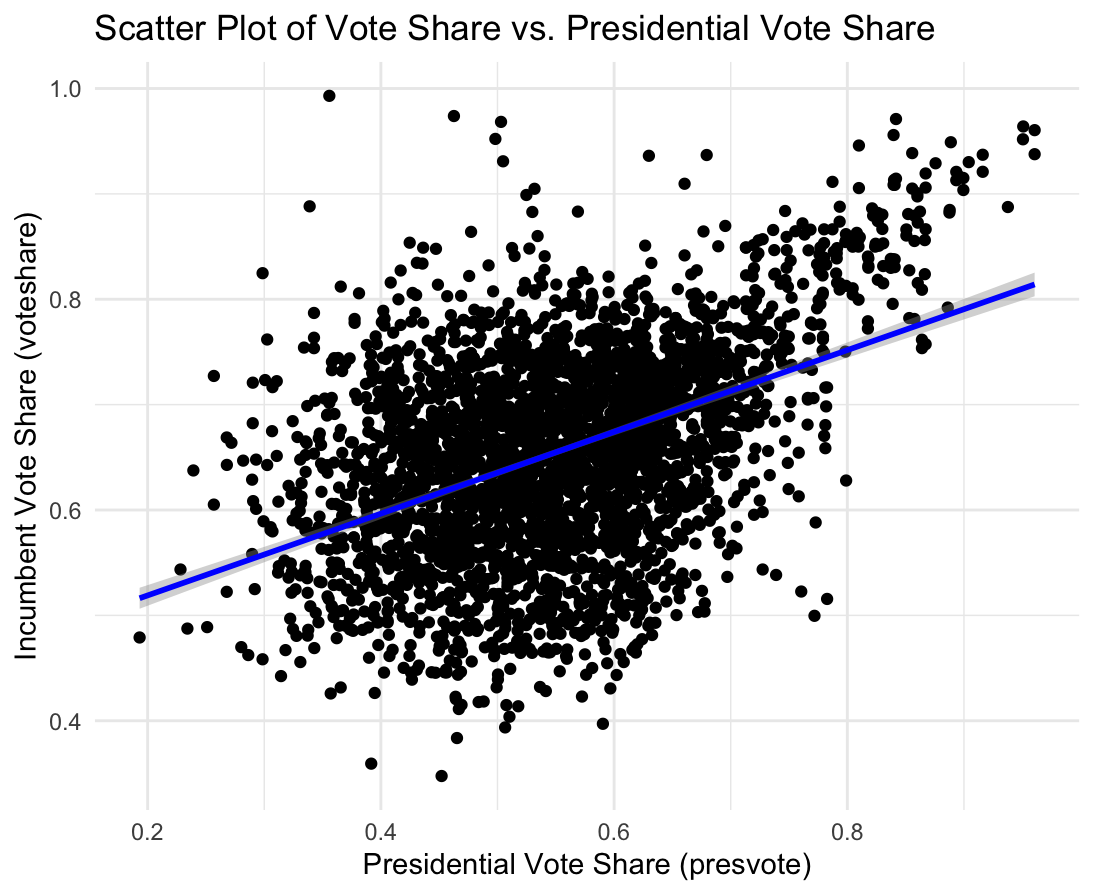
\includegraphics[width=.80\textwidth]{Scatterplot_4.2.png}
		\item Write the prediction equation.
		 \lstinputlisting[language=R, firstline=128, lastline=133]{PS3_Lyu_Jia.R}
		 \begin{verbatim} 
		 voteshare = 0.441  +  0.388 * presvote
		\end{verbatim}	
	\end{enumerate}
	


\section*{Question 5}
\noindent What if the incumbent's vote share is affected by both the president's popularity and the difference in spending between incumbent and challenger? 
	\begin{enumerate}
		\item Run a regression where the outcome variable is the incumbent's \texttt{voteshare} and the explanatory variables are \texttt{difflog} and \texttt{presvote}.	
		\lstinputlisting[language=R, firstline=137, lastline=139]{PS3_Lyu_Jia.R} 
		\begin{verbatim}
		Call:
		lm(formula = voteshare ~ difflog + presvote, data = df)
		
		Residuals:
		Min       1Q   Median       3Q      Max 
		-0.25928 -0.04737 -0.00121  0.04618  0.33126 
		
		Coefficients:
		Estimate Std. Error t value Pr(>|t|)    
		(Intercept) 0.4486442  0.0063297   70.88   <2e-16 ***
		difflog     0.0355431  0.0009455   37.59   <2e-16 ***
		presvote    0.2568770  0.0117637   21.84   <2e-16 ***
		---
		Signif. codes:  0 ‘***’ 0.001 ‘**’ 0.01 ‘*’ 0.05 ‘.’ 0.1 ‘ ’ 1
		
		Residual standard error: 0.07339 on 3190 degrees of freedom
		Multiple R-squared:  0.4496,	Adjusted R-squared:  0.4493 
		F-statistic:  1303 on 2 and 3190 DF,  p-value: < 2.2e-16
	\end{verbatim}	
	\begin{verbatim}
		
The regression analysis reveals a significant positive relationship 
between the incumbent's vote share, campaign spending difference
(`difflog`), and the president's vote share (`presvote`). A one-unit
increase in `difflog` results in a 0.0355 increase in the incumbent's 
vote share, while a one-unit increase in `presvote` results in a 0.2569  
increase. The model explains 44.96% of the variation in vote share
R-squared = 0.4496), with an F-statistic of 1303 and p-value 
< 2.2e-16, indicating statistical significance. However, other factors 
may still influence the incumbent's vote share.
	\end{verbatim}	
		
		\item Write the prediction equation.
		\lstinputlisting[language=R, firstline=141, lastline=148]{PS3_Lyu_Jia.R} 
		\begin{verbatim}
		voteshare = 0.449  +  0.036 * difflog  +  0.257 * presvote
		 \end{verbatim}	
		 
		\item What is it in this output that is identical to the output in Question 4? Why do you think this is the case?
			\begin{verbatim}
Similarities:
1. Residuals:The statistical data for residuals in both models are identical:
minimum value: -0.25928, first quartile: -0.04737, median: -0.00121,
third quartile: 0.04618, and maximum value: 0.33126.
2. Residual Standard Error:The residual standard errors are nearly
identical (0.07339 and 0.07338), indicating similar model fits.
3. F-statistic and p-value:Both models show significant F-statistics 
and p-values, suggesting they are statistically significant.
		
Reasons:
1. Same Dataset:Both models use the same dataset, resulting in similar
residual distributions.
2. Similar Error Structures:The error terms in both models likely follow
similar distributions.
3. Same Sample Size:The similar degrees of freedom (3190 and 3191)
contribute to comparable residual standard errors.
4. Model Significance:Both models effectively explain the variability in the
dependent variables, supported by significant F-statistics.
5. Linear Relationships: Both models capture linear relationships, leading
to similar residual patterns.
6. Random Error: In large samples, random error can produce similar
residual patterns, even with different models.
	\end{verbatim}	
		
	\end{enumerate}




\end{document}
